\section{Bevægelsesanalyse}
%Indhold:
%- Hvad er bevægelse
%	- definition og opståen 
%- Hvordan måles bevægelse
%- Karakteristika for forskellige bevægelser 
%	- Sammenligning af de forskellige aktiviteter
%		- hvordan adskiller de sig fra hinanden
%
\textit{Følgende afsnit indeholder bevægelsesanalyser for gang, løb og cykling. Dette medhenblik på at finde karakteristika for de tre aktivitetsformer og hvorledes deres forskelle senere vil kunne være behjælpelige i forbindelse med detektering af de enkelte aktiviteter. Der vil derfor afslutningsvist være en sammenligning af karakteristika for de tre aktiviteter}

\subsection{Gang}
Gang er en fysisk aktivitet kendetegnet ved altid at have et ben på jorden. Aktiviteten betegnes som en cyklus, da den samme række bevægelser gentages for at udføre aktiviteten. Bevægelserne er desuden identiske for højre og venstre ben, men forskudt med en halv cyklus, hvorfor bevægelsen kun vil blive beskrevet for højre ben. \citep{VaughanDavisOConnor1992,Whittle1990} 

En gangcyklus inddeles i to faser, standfasen og svingfasen, hvilket fremgår af \figref{fig:gang_cyklus}. Standfasen har en varighed svarende til cirka 60\% af en gangcyklus, og påbegyndes idet den højre fod opnår kontakt med underlaget. Fasen indebærer den tid hvor højre fod er i berøring med jorden. Svingfasen udgør derimod cirka 30\% af hele gangcyklussen, og er den periode, hvor foden og benet bevæges frem og derfor ikke er i berøring med jorden. Efter denne fase, er foden igen klar til isætning af højre hæl. \citep{VaughanDavisOConnor1992}

\begin{figure}[H]
	\centering
	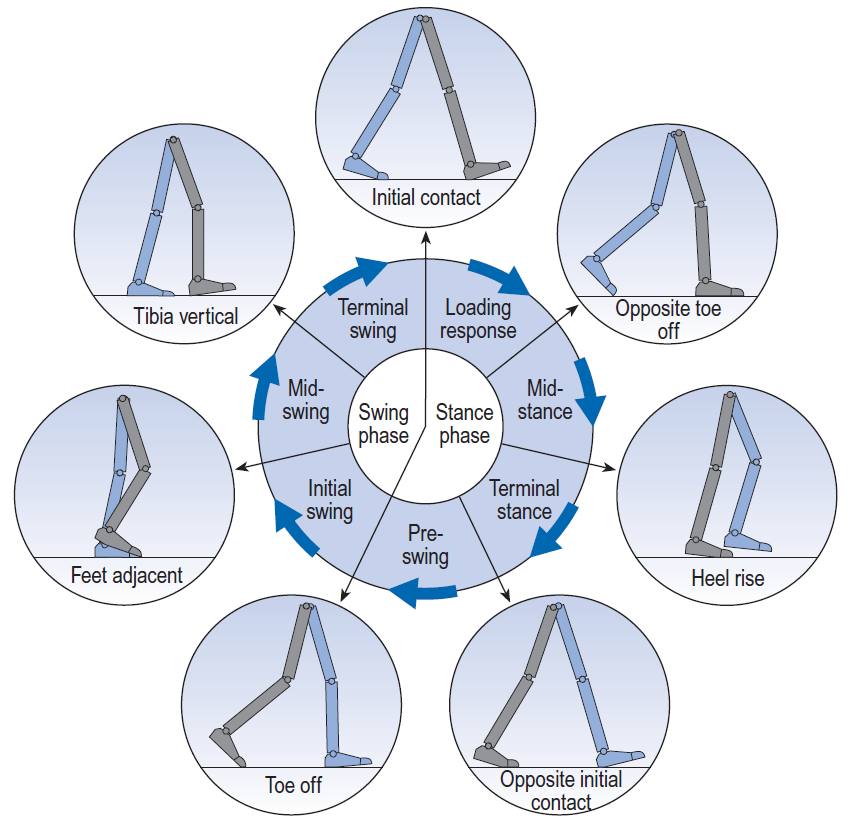
\includegraphics[scale=0.5]{figures/bProblemloesning/gang_cyklus2.png}
	\caption{På figuren ses en gangcyklus opdelt i standfase og svingfase. \citep{Whittle1990} (Modeficeret)}
	\label{fig:gang_cyklus}
\end{figure}
\fxnote{Opg: SKAL MODIFICERES. Gør så at figuren også har den procentvise fordeling af faserne på}
	
Som det fremgår af billedet, er standfasen og svingfasen yderligere inddelt henholdsvis i 5 og 3 faser. \newline
Standfasens første fase er et hæl-nedslag, som starter hele cyklussen, hvilket opnås når den højre hæl kommer i kontakt med jordoverfladen. Herefter er foden flad og den venstre fod er derimod i berøring med overfladen med tåspidserne. Hælen på den højre fod løftes nu, alt i mens den venstre fod, som er i svingfasen, passerer den højre fod. Der opstår nu et hæl-slip for den højre fod, og der skabes en berøring af den venstre fod på underlaget. Standfasen afsluttes med en fleksion af anklen og dermed et afsæt fra tæerne på højre fod. \newline
Den højre fod, og det højre ben, er dermed i svingfasen, som påbegyndes med en acceleration af foden og benet. Denne acceleration begynder når foden ikke længere har kontakt med underlaget i standfasen. Derfor vil det højre ben blive bevæget frem mod det venstre ben. Efterfølgende vil der være et såkaldt, midt-sving som forekommer når højre fod er lige under kroppen og dermed ud for den venstre fod, som er i kontakt med jorden. Afsluttende for svingfasen er der en deacceleration. Denne fase involverer en række muskler som sænker hastigheden af benet og fodens fremadgående bevægelse, således kroppen er klar til det kommende hæl-nedslag i standfasen.


\subsection{Løb}
Løb er en aktivitet karakteriseret ved, at kun én fod rør jorden ad gangen. Denne aktivitet beskrives, ligesom gang, som en cyklus der gennemgår forskellige faser. Denne aktivitet karakteriseres som en hurtigere variation af gang, hvor kun én fod rør jorden ad gangen. Løbecyklussen består derfor af fire faser, som vist på \figref{fig:loebecyklus}: standfasen, den første svævefase, svingfasen og den anden svævefase. \citep{Adelaar1986,Novacheck1998}

\begin{figure}[H]
	\centering
	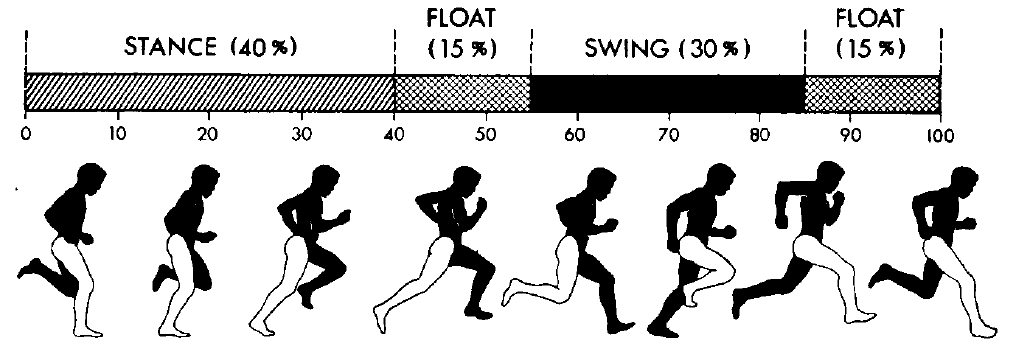
\includegraphics[scale=0.4]{figures/bProblemloesning/loeb_cyklus1.png}
	\caption{På figuren ses en løbecyklus opdelt i standfase, svingfase og to svævefaser. \citep{Adelaar1986} (Modeficeret}
	\label{fig:loebecyklus}
\end{figure}
\fxnote{Opg: SKAL MODIFICERES}

På samme vis som ved gangcyklussen, initieres løbecyklussen idet den højre hæl rammer jorden, hvilket er begyndelsen af den første fase, standfasen, som udgør 40\% af løbecyklussen. Herefter fortsætter foden til midt stand, hvor den står fladt på jorden, og afslutningsvis udføres et accelererende afsæt med tæerne, hvilket leder op til den næste fase, den første svævefase. \newline
De to svævefaser, som går igen to gange i løbecyklussen, er identiske og udgør hver 15\% af cyklussen. Disse er karakteriseret ved at begge ben er løftet fra jorden. \newline
Mellem de to svævefaser, er svingfasen, som udgør 30\% af løbecyklussen. Denne fase begynder idet foden hæves og knæet føres frem, hvorefter hælen igen sænkes, dette sker mens den venstre fod udfører standfasen, hvorved denne fase er supportet af en fod i jorden. Efter denne fase udføres anden svævefase før en ny cyklus kan påbegyndes. \citep{Adelaar1986,Novacheck1998}

Løb er karakteriseret ved, at kun én fod rør jorden ad gangen. Dette resulterer i at der er et større stress på leddene ved løb i forhold til gang. Eksempelvis vil en person på 68 kg have et stress på sin fod på 35 kg/m ved gang, mens det ved løb vil være et stress på 110 ton/m. \citep{Adelaar1986}\fxnote{Opg: mere om dette!}

\fxnote{Opg: Tjek bog om der er mere eller om det muligvis er en bedre/nyere kilde}



\subsection{Cykling}





\subsection{Karakteristika for de tre aktivitetsformer}
%På baggrund af dette afsnit skal vi kunne lave en kode som kan adskille aktiviteterne.



De tre forskellige aktivitetsformer har en række karakteristika som adskiller dem fra hinanden men også flere fællestræk. \newline 
Gang er en aktivitet karakteriseret som en cyklus, hvor der altid er én eller to fødder i jorden. Denne cyklus er udgjort af to faser, en standfase og en svingfase, som hver udgør henholdsvis 60\% og 40\%.
Faserne for højre og venstre fod er identiske, men forskudt med en halv cyklus, hvilket resulterer i at standfasen for højre og venstre fod vil overlappe hinanden. Herved vil personen to gange i cyklussen have begge fødder i jorden samtidig. \newline
Det er ikke et så stort stress på fødderne ved gang, da det ikke går betydelig hurtigt, og da der altid er mindst en fod i jorden på en gang, hvorved en person ikke vil starte standfasen med at sætte en hæl i jorden som skal bære hele deres kropsvægt (ganget med hastigheden).\fxnote{Vi skulle gerne finde mere om dette og kunne skrive mere om det oppe i afsnittet - dette skal rettes til på baggrund af det som bliver skrevet.}

Løb er i grundtræk meget lignende gang, blot hurtigere; fod- og benbevægelser er ens for gangcyklussen og løbecyklussen. Da løb går betydelig hurtigere er der i denne cyklus to faser, som ikke optræder ved gang, svævefaser, hvor begge fødder er hævet fra jorden. Standfasen og svingfasen er derfor kortere ved løb og udgør henholdsvis 40\% og 30\%, mens de to svævefaser hver udgør 15\%. \newline
I denne fase er der ikke altid en fod i jorden, og det er maksimalt én fod i jorden, hvilket gør at en person vil få et større stress på fodden idet hælen isættes i starten af standfasen sammenlignet med gang.\fxnote{Vi skulle gerne finde mere om dette og kunne skrive mere om det oppe i afsnittet - dette skal rettes til på baggrund af det som bliver skrevet.}

Hvis hastigheden øges til en spurt i stedet for løb, er cyklussen den samme, dog ændres længden af faserne. Standfasen og svingfasen reduceres mens svævefaserne øges. \citep{Lee1998}\fxnote{Opg: Skal vi have mere om dette, det virker måske lidt kort.}

Cykling adskiller sig betydeligt mere fra gang og løb, da denne er en konstant cyklus, og dermed ikke er opdelt i faser. Fødderne og benene udfører en cirkulær bevægelse...




